\section{Motivation}
\label{sec:motivation}

In this section, with help of a bank account example, we motivate the
need for a framework to express and enforce fine-grained
application-level consistency requirements under weak consistency
models. 
% \GK{The following text needs to be polished}

% We assume a system model where the eventually consistent database is organized
% as a collection of key-indexed, object-valued tables. The objects stored in the
% tables are instances of the same replicated data type. The database is composed
% of a number of \emph{replicas}, and each object is fully replicated across all
% the replicas. Under this model, a client request for an operation with no
% application-level consistency requirement can be serviced if at least one of
% the replicas is reachable. Thus, with the addition of new replicas, and placing
% them close to the clients, leads to improved throughput and reduced latencies.

\subsection{Bank account database}

Suppose our goal is to implement a highly available bank account
service on top of an eventually consistent data store. For the sake of
presentation, we restrict ourselves to bank account objects (records)
with following simple schema:

\begin{codesql}
Create Table BankAccount (
  accountNo int PRIMARY KEY,
  balance float CHECK (balance >= 0))
\end{codesql}

\noindent and with support for the following \emph{operations}:

\begin{codehaskell}
type AccountNo = Int
type Amount = Float
getBalance :: AccountNo -> Amount
deposit    :: AccountNo -> Amount -> ()
-- returns false if the account has insufficient balance
withdraw   :: AccountNo -> Amount -> Bool
\end{codehaskell}

\begin{figure}[t]
\centering
\subfigure[Unsafe Withdraw]{\label{fig:unsafeWithdrawAnomaly}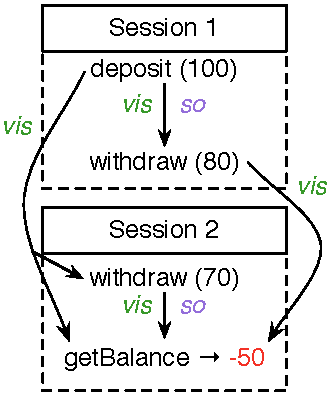
\includegraphics[width=0.31\columnwidth]{Figures/Motivation4}}
\hfill
\subfigure[Negative Balance]{\label{fig:negativeBalanceAnomaly}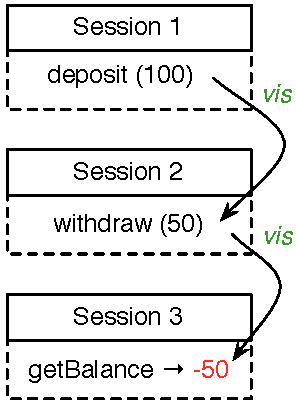
\includegraphics[width=0.31\columnwidth]{Figures/Motivation2}}
\hfill
\subfigure[Missing update]{\label{fig:missingUpdateAnomaly}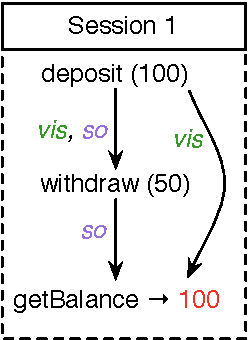
\includegraphics[width=0.26\columnwidth]{Figures/Motivation1}}
%\hfill
%\subfigure[Monotonicity violation]{\label{fig:monotonicityAnomaly}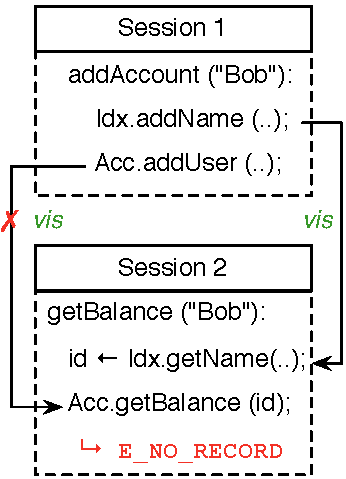
\includegraphics[width=0.36\columnwidth]{Figures/Motivation3}}
\caption{Anomalies possible under eventual consistency for the get balance operation.}
\label{fig:cleanliness_examples}
\end{figure}

The sole attribute of a \cf{BankAccount} object, identified by its unique
\cf{accountNo}, is its current \cf{balance}. A \cf{deposit} operation
on a \cf{BankAccount} adds some \cf{Amount} to its \cf{balance},
whereas a \cf{withdraw} operation subtracts. Operation \cf{getBalance}
returns the current \cf{balance} in the account. A \cf{withdraw}
operation succeeds and returns \cf{True} only if there is sufficient
balance in the account. Otherwise, it fails and returns \cf{False}. 

If we were to use a traditional database system to store
\cf{BankAccount} objects, all that needs to be done is to define the
\cf{BankAccount} schema, as shown above. The database management
system effectively sequentializes all accesses to the database, and
automatically enforces the required integerity constraints on the
data, so that it is never possible for a \cf{getBalance} operation to
return a negative balance, or for a \cf{withdraw} to succeed without
having sufficient balance in the account. However, under eventual
consistency, such anomalies are bound to occur as demonstrated in the
following subsection. 


\subsection{Anomalies}

Consider the execution shown in fig.~\ref{fig:negativeBalanceAnomaly}.
Assume that all operations in the figure are on the same
\cf{BankAccount} object. Execution contains two concurrent client
sessions, where one of the sessions executes a \cf{withdraw} followed
by a \cf{getBalance} operation. We say that \c{withdraw} precedes
\cf{getBalance} in \emph{session order}, and visualize it as a
directed \cf{so} edge from the former to the later. Edges labelled
\cf{vis} in the figure capture the \emph{visibility} relation between
operations; an operation is said to be \emph{visible} to other
operation if the later can witness the effects of the former. Two
operations that are not related either via \cf{vis} or \cf{so} are
said to be concurrent. The figure shows an execution where concurrent
\cf{withdraw}s in different sessions succeed independently, but a
subsequent \cf{getBalance} operation that witnesses both the
\cf{withdraw}s reports a negative balance. 

It is easy to see that the only way to ensure that integrity
constraint on \cf{balance} is to prevent concurrent withdrawls on the
\cf{BankAccount}. This can be done by insisting that \cf{withdraw} be
executed with strong consistency. Although this prevents unsafe
withdrawls from going through, a strongly consistent \cf{withdraw}
itself is not sufficient to prevent \cf{getBalance} from ever
reporting a negative balance to the end user.

Consider the execution shown in fig.~\ref{fig:negativeBalanceAnomaly},
which consists of three concurrent sessions performing a \cf{deposit},
a \cf{withdraw}, and a \cf{getBalance}, respectively, on the same
\cf{BankAccount}. Assume that initial balance in the account is zero.
As the \cf{vis} edge indicates, operation \cf{withdraw(50)} in session
2, can witnesses the effects of \cf{deposit(100)} from session 1,
leading it to rightfully conclude that the current balance is 100.
Consequently, \cf{withdraw(50)} is performed safely. The effect of
this \cf{withdraw} operation subsequently becomes visible to the
\cf{getBalance} in Session 3. However, \cf{getBalance}, which can only
see the effect of \cf{withdraw} from session 2, but not \cf{deposit}
from session 1, reports the balance of negative 50 to the user.

Negative balance is not the only inconsistency that the user is
exposed to under an eventually consistent bank account. Figure
~\ref{fig:missingUpdateAnomaly} shows an execution where
\cf{getBalance} operation in a session does not witness the effects of
\cf{withdraw} operation performed in the same session, possibly
because \cf{getBalance} was served by a replica that hasn't yet merged
the \cf{withdraw} effect, which could have been served by a different
replica. This anomaly leads the user to incorrectly conclude that the
\cf{withdraw} operation failed to go through.

Although it is easy to understand the reasons behind the occurance of
the aforementioned negative balance and missing update anomalies, the
fix is not quite apparent. Making \cf{getBalance} a strongly
consistent operation is definitely sufficient to avert anomalies, but
is it really necessary? Given that a strongly consistent operation is
significantly expensive, both in terms of latency and monetary value, we ideally
would not want to request strong consistency, unless there are
no alternatives available. Unfortunately, this requires us to
understand subtle differences in semantics of various kinds of weak
consistency alternatives, such as timeline consistency and session
guarantees, offered by off-the-shelf eventually consistent data
stores. This process is error-prone, and becomes further complicated
in presence of transactions, as demonstrated in Sec.
~\ref{sec:transactions}.


\subsection{Implementation in Quelea}

\name automates this error-prone task by letting the programmer
declare application-level consistency constraints as \emph{contracts},
obviating the need to understand store-level consistency guarantees,
and relieving programmer from having to match application
requirements with appropriate store-level alternatives. The
cornerstone of declarative reasoning in \name is the programming model
built around operation-based CRDTs~\cite{shapiroCRDT}. A replicated
data type in \name is defined as a tagged union type, where each tag
is the name of a unique operation defined on the data type. 
%types in Quelea are defined as reductions over the set of effects.
%The following data type definitions capture the operations and effects
%on the bank account and user index objects.
For example, following is the definition of the \cf{BankAccount}
data type in \name:
\begin{codehaskell}
data BankAccount =  Deposit Float | Withdraw Float 
                 | GetBalance
\end{codehaskell}

In Quelea, an object state is nothing but the set of effects (called
the \emph{context}) on this object. As such, \cf{Deposit} and
\cf{Withdraw} effects simply include the amount deposited or
withdrawn, and \cf{AddUser} effect includes the user name. Similarly,
on the user index table, where the key is user name, the value is
simply an effect (\cf{AddName}) binding some user id at this key.
\cf{GetBalance} and \cf{GetName} correspond to the corresponding
read-only operations. The complete definition of the operations on
bank account and user index objects is given below.

\begin{codehaskell}
-- Get balance takes no arguments and read-only
getBalance :: [BankAcc] {- context -} -> () {- args -}
  -> (() {- ret val -}, Maybe BankAcc {- effect -})
getBalance ctxt _ = (sum [v | Deposit v (- ctxt]
        - sum [v | Withdraw v (- ctxt], Nothing)

-- withdraw returns True on success
withdraw :: [BankAcc] -> Float -> (Bool, Maybe BankAcc)
withdraw c v = if sel1 $ getBalance c () >= v
               then (True, Just $ Withdraw v)
               else (False, Nothing)

deposit :: [BankAcc] -> v -> ((), Maybe BankAcc)
deposit _ v = ((), Just $ Deposit v)

addUser :: [BankAcc] -> UserName -> ((), Maybe BankAcc)
addUser _ n = ((), Just $ AddUser n)

addName :: [UserIdx] -> UserID -> (Bool, Maybe UserIdx)
addName [] uid = (True, Just $ AddName uid)
addName x:_ _ = (False, Nothing)

getName :: [UserIdx] -> ()
        -> (Maybe UserName, Maybe UserIdx)
getName [] _ = (Nothing, Nothing)
getName (AddUser uid:_) _ = (Just uid, Nothing)
\end{codehaskell}

The definitions are a straight forward encoding of the expected behavior.
Quelea programming model provides the programmer complete freedom regarding the
semantics and desired convergence property of the replicated data type, and
indeed, we can encode the well-known CRDTs~\cite{SSS} in a declarative fashion.
Observe that the operation definitions presented here only capture the
convergence properties of the replicated data type, and are not concerned with
the consistency properties, which is expressed through the contract language.

\subsection{Contracts}

The contract for the strongly consistent \cf{addName} operation is given below:
\begin{smathpar}
\begin{array}{l}
\rsf{addNameCtrt} = \forall (a:\rsf{AddName}). \\
\qquad \sameobj{a}{\cureff} \Rightarrow \vis{a}{\cureff} \vee \vis{\cureff}{a} \vee a = \cureff
\end{array}
\end{smathpar}

In the above definition, $\cureff$ represents the current effect --- the effect
emitted by the \cf{addName} operation. The contract simply states our
high-level observation; for any effect $a$ which is also an \cf{AddName} effect
on the same object, it must be the case that $a$ is visible to $\cureff$ or
vice verse, or $a$ is $\cureff$. Here, $\sameobjZ$ and $\visZ$ are primitive
relations. This contract ensures that any two \cf{addName} operations will be
seen by each other. The contract for withdraw is similar to the
\cf{addNameCtrt}.

Since the deposit operation does not have any restrictions, its contract is
simply $\true$. Same is the case for \cf{addUser} operation. The contract for
get balance operation is:
\begin{smathpar}
\begin{array}{l}
\rsf{getBalCtrt} = \forall (a:\rsf{Deposit}), (b:\rsf{Withdraw}). \\
\qquad \vis{a}{b} \wedge \vis{b}{\cureff} \Rightarrow \vis{a}{\cureff} \\
\qquad \vee (\soZ \cap \sameobjZ) (a,\cureff) \Rightarrow \vis{a}{\cureff} \\
\qquad \vee (\soZ \cap \sameobjZ) (b,\cureff) \Rightarrow \vis{b}{\cureff}
\end{array}
\end{smathpar}

If a withdraw $b$ is visible to the get balance operation, then all deposit
operations $a$ visible to withdraw should be visible to the get balance
operation. This prevents negative balance anomalies. The rest of the contract
says that a get balance operation must witness previous deposit and withdraw
operations on the same object in the same session. This prevents missed update
anomalies.

Similar to contracts on operations, Quelea supports contracts on transactions.
The contract on the \cf{getBalanceName} transaction is given below:
\begin{smathpar}
\begin{array}{l}
\rsf{getBalanceNameCtrt} = \forall (a:\rsf{GetName}), (b:\rsf{GetBalance}), \\
\quad (c:\rsf{AddName}), (d:\rsf{AddUser}). ~\trans{a}{b}{c}{d} \wedge \so{a}{b} \\
\qquad \wedge ~\vis{c}{a} \wedge \sameobj{d}{b} \Rightarrow \vis{d}{b}
\end{array}
\end{smathpar}

$\trans{a}{b}{c}{d}$ says that the action pairs $a,b$ and $c,d$ are in the same
transaction, and the two transactions are distinct. The contract says
specifically forbids the anomaly presented in
Figure~\ref{fig:monotonicityAnomaly}. This is the desired semantics for the
\cf{getUserName} transaction.

The programmer simply defines such contracts on the operations and the
transactions. Quelea logically analyzes the contracts, and maps the
corresponding operation to the precise store consistency and isolation level.
Thus, Quelea equips the programmer with a declarative model for reasoning and
expressing eventually consistent programs.
